\newpage
\chapter{Implementation}
\section{Problem}


Forward the message to the specified client.
With the help of java suckt it is possible to establish a connection between the server and a client. Through this connection the client and the server can communicate with each other. 
The client can send a message to the server, and the server can also reply to the client and send retransmissions.

The difficulty is that the client sends the messages to the other client. 
In this case, the message must be sent from the first client to the server, and then the messages must be forwarded from the server to the correct client. 
After that, the other client must send the response back to the first client via the server.

\section{Solution}


After a lot of thinking, a solution was found to use the Thread class.
The thread class must be implemented for client and server, so that the server receives the messages
from the first client and at the same time forwards them to the right client and vice Versa.
the thread for the client starts to call the method onReceive as rekrusion so that the client is
always ready to receive the messages

\section{Server GUI}

In the server mask you can enter a server with its IP address and port (As default 127.0.0.1:8080)
and then click the Start server button to start the server. 
When the server is started, two tables will display all connected clients and all created groups, respectively.
If you click on the Client tab, a table with the following columns will be displayed (checked, username, host, port).
\medskip

\noindent
The column with the check boxes are used to select the clients to be deleted. 
After the clients are selected, you should click the "Delete" button under the table.

\begin{figure}
    \centering
    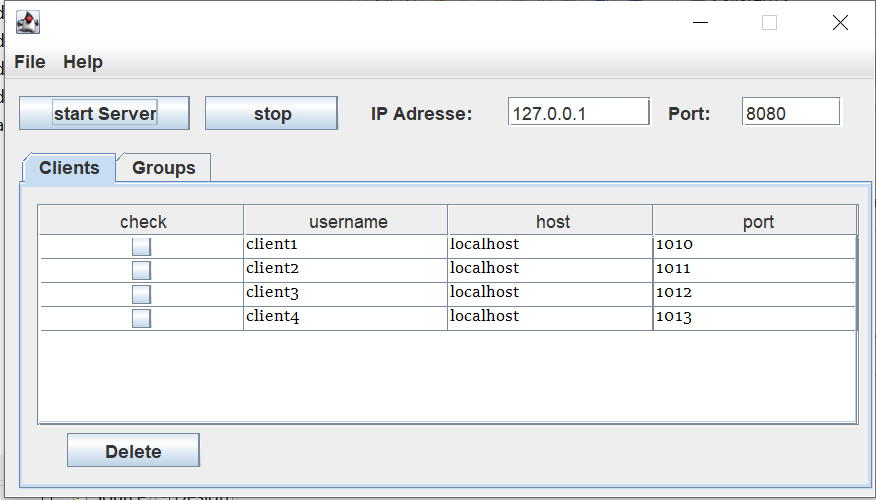
\includegraphics[width=0.7\textwidth]{gfx/GUI_Server_Clients.png}
    \caption{GUI-Server-Clients}
    \label{fig:gui-server-clients}
\end{figure}

\noindent
The "Groups" table has less columns than the "Clients" table, namely (Check, Name of the group, count of clients )
The "Check" column has the same principle of operation as in the "Clients " table,
the groups can be selected to be deleted. 

\begin{figure}
    \centering
    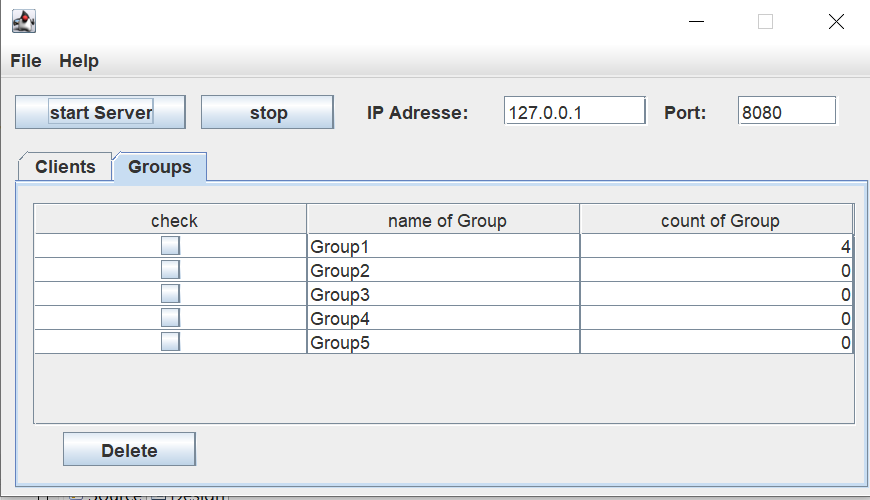
\includegraphics[width=0.7\textwidth]{gfx/GUI_Server_Groups.png}
    \caption{GUI-Server-Groups}
    \label{fig:gui-server-groups}
\end{figure}

\noindent
when a client is deleted, a message is sent to all other clients with the content (the client is deleted with server).
This message (the Group is deleted with serve) is also sent for all clients when a group is deleted. 
\medskip

\noindent
If you want to stop the server, it must click on the "Stop" button at the top of the mask.
when you want to close the server application, click on File -->Exit.
